\documentclass[10pt,twocolumn,letterpaper]{article}

% \documentclass[12pt,letterpaper]{article}
\usepackage{stfloats}
\usepackage{lipsum}
\usepackage{cite}
\usepackage{multicol}
\usepackage{listings}
\usepackage{titlesec}
\setcounter{secnumdepth}{4}
\usepackage{times}
\usepackage{epsfig}
\usepackage{graphicx}
\usepackage{amsmath}
\usepackage{amssymb}
\usepackage{subfig}
\usepackage{abstract}
\usepackage[toc,page]{appendix}

\renewcommand{\abstractnamefont}{\normalfont\Large\bfseries}
\renewcommand{\abstracttextfont}{\normalfont\normalsize\it}
\setlength{\absleftindent}{0pt}
\setlength{\absrightindent}{0pt}

\titleformat{\paragraph}
{\normalfont\normalsize\bfseries}{\theparagraph}{1em}{}
\titlespacing*{\paragraph}
{0pt}{3.25ex plus 1ex minus .2ex}{1.5ex plus .2ex}

% Include other packages here, before hyperref.

% If you comment hyperref and then uncomment it, you should delete
% egpaper.aux before re-running latex.  (Or just hit 'q' on the first latex
% run, let it finish, and you should be clear).
\usepackage[breaklinks=true,bookmarks=false]{hyperref}

% \cvprfinalcopy% *** Uncomment this line for the final submission

% \def\cvprPaperID{****} % *** Enter the CVPR Paper ID here
\def\httilde{\mbox{\tt\raisebox{-.5ex}{\symbol{126}}}}
\graphicspath{{./pics/}} % put all graphics here

% Pages are numbered in submission mode, and unnumbered in camera-ready
%\ifcvprfinal\pagestyle{empty}\fi
%\setcounter{page}{4321}
\begin{document}

%%%%%%%%% TITLE
% \title{\LaTeX\ Author Guidelines for CVPR Proceedings}
\title{Model Pruning}
\author{Patricia Gschoßmann\\
	Technical University Munich\\
	Munich, Germany\\
	{\tt\small patricia.gschossmann@tum.de}}

\maketitle
%\thispagestyle{empty}

%%%%%%%%% ABSTRACT
\begin{abstract}
	\noindent
	This paper proposes a novel filter pruning framework for structured pruning with predefined target network architectures and without the need for fine-tuning.
	The main purpose behind this is to encode the input data to solve the problem of data storage, transmission and processing for autonomous vehicles.
	It can be shown, that directly training the small target model from random initialization can achieve similar performance, as the model obtained from the standard pruning three-stage pipeline.
	However, the setup used can still be adapted in order to improve results.
\end{abstract}

%%%%%%%%% BODY TEXT
\section{Introduction}
Network Pruning tackles some of the major challenges of deep learning these days:
Today's deep learning models are gaining more and more accuracy but are sacrificing fast execution times, low power consumption and storage space in the process.\footnote{\url{https://towardsdatascience.com/pruning-deep-neural-network-56cae1ec5505}}
This especially limits the applications for real-time inference and low-resource settings as in autonomous driving.
Thus, smaller networks with an optimal number of parameters are more desired than networks with more parameters than necessary.\\\\
The typical pruning algorithm is a three-stage pipeline, i.e., training, pruning and fine-tuning (see fig.~\ref{fig:standard_pruning}).
During pruning, weights are ranked according to a certain criterion (e.g. L1-norm~\cite{Li2017}).
In each layer, a certain percentage of filters with smaller L1-norm will be pruned while the remaining are kept to best preserve the accuracy.
The newly obtained model is retrained to recover the original performance as far as possible.
The procedure is stopped, once the performance drops below a certain threshold.\\
This paper proposes a novel filter pruning framework for structured pruning with predefined target network architectures and without the need for fine-tuning.
It can be shown, that directly training the small target model from random initialization can achieve similar performance, as the model obtained from the three-stage pipeline.
This shows that the obtained number of parameters is more meaningful than the preserved original weights.\\\\
The paper is structured as follows:
\begin{itemize}
\item Section~\ref{sec:methodology} describes the structure and procedure of the novel pruning framework proposed in this paper.
\item Section~\ref{sec:related_work} provides a summary of previous research on alternative model compression and pruning techniques.
\item In section~\ref{sec:experiments} the results of the most successful experiments are presented and evaluated.
	Additionally, failed attempts are analyzed.
\item Finally, the work is summarized in section~\ref{sec:conclusion} and an outlook on future research possibilities is given.
\end{itemize}

\begin{figure}[hpbt]
	\centering
	\includegraphics[scale=0.15]{pics/standard_pruning.png}
	\caption[]{Standard model pruning pipeline (figure taken from~\cite{Mart2020}).
	}
	\label{fig:standard_pruning}
\end{figure}

\section{Methodology}\label{sec:methodology}
\begin{figure}[hpbt]
	\centering
	\includegraphics[scale=0.125]{pics/new_approach.png}
	\caption[]{Rough sketch of the new pruning approach (figure taken from~\cite{Khan2020}).
		During pruning intermediate model with two separate branches is used, each corresponding to the original model and the smaller target model.
		The output is the weighted sum of both branches.
		$\alpha$ is reduced iteratively from 1 to 0.
	}
	\label{fig:new_approach_highlevel}
\end{figure}
\noindent Fig.~\ref{fig:new_approach_highlevel} depicts a high-level sketch of the proposed model pruning approach.
The technique aims to directly train a pruned target model without intermediate fine-tuning steps.
The key feature of this approach is that the original model with pre-trained weights is preserved during the pruning process and serves as a back-up in case the pruned model's performance drops.
At first, an intermediate network is constructed based on the original model's architecture.
For each original layer to prune an additional parallel branch is added with the desired number of parameters.
The intermediate model's output is the weighted sum of both branches,
A weighting factor $\alpha$ is introduced to compute this sum.
During pruning $\alpha$ is reduced iteratively from 1 to 0.
One question that needs to be answered is how to schedule $\alpha$.\\
If successful, the performance should be maintained as good as possible, after reaching $\alpha=0$.
The next step is to shrink the intermediate model, i.e. to remove the original branch.
This is done using the so-called Einstein summation\footnote{https://pytorch.org/docs/stable/generated/torch.einsum.html}.
New, smaller weights with the desired number of parameters are obtained.\\\\
When constructing a parallel branch, it must be taken into account that no non-linear activation function may occur at the beginning or end in order for this approach to work, as depicted in fig.~\ref{fig:new_approach_detail}.
If done correctly, both layers - the one to be pruned and the first layer in the parallel branch (Conv1 and ConvA in fig.~\ref{fig:new_approach_detail}) - can be combined into one, as they are only two consecutive linear operations.
The same applies to the last layer in the parallel branch and the layer after the one to be pruned (ConvB and Conv2 in fig.~\ref{fig:new_approach_detail}).\\
Furthermore, the parallel branch's architecture is dependent on the type of layers occurring in the original model, since the weights of two different layers cannot be mathematically combined with each other.
Fig.~\ref{fig:new_approach_detail} shows an exemplary application of the framework on two consecutive convolutional layers.
\begin{figure}[!h]
	\centering
	\subfloat[Original model.
	Output and input channels marked in red should be reduced.]{\includegraphics[scale=0.1]{pics/original_model.png}}
	\hspace{10pt}
	\subfloat[Intermediate model with parallel branches.
	Output and input channels marked in blue are merged through the weight multiplication.]{\includegraphics[scale=0.1]{pics/parallel_branches.png}}
	\hspace{10pt}
	\subfloat[Pruned model after multiplication.
	Reduced output and input channels are marked in red.]{\includegraphics[scale=0.1]{pics/pruned_model.png}}
	\caption[]{Detailed view of the new pruning approach on two consecutive convolutional layers.
		For each original layer to prune an additional parallel branch is added with the desired number of parameters.
		After reaching $\alpha=0$ the original branch is removed by multiplying Conv1 with ConvA and ConvB with Conv2 using the so-called Einstein summation\footnote{https://pytorch.org/docs/stable/generated/torch.einsum.html}.
		New, smaller weights with the desired number of parameters are obtained.
	}
	\label{fig:new_approach_detail}
\end{figure}

\section{Related Work}\label{sec:related_work}
Luo et al.~\cite{Luo2017} prune a channel based on the outputs of its next layer, not its own.
In more detail, the channels that have the smallest effects on the next layer's activation values are removed.\\
Similarly, He et al.~\cite{He2017} propose an regression based channel selection and least squares reconstruction technique that prunes each layer by minimizing the feature map reconstruction error of the next layer.\\
Liu et al.~\cite{Liu2017} use a method called network slimming to identify unimportant channels during training.
This is done by multiplying the output of each channel with an individual scaling factor $\gamma$.
The network weights and scaling factors are trained, with sparsity regularization imposed on the latter.
% A sparsity-induced penalty on the scaling factors are added to the normal training loss.
Channels with small factors are removed followed by fine-tuning the pruned network.
They were able to decrease the computational cost of state-of-the-art networks up to 20$\times$ with no accuracy loss.\\
The Multi-Dimensional-Pruning framework from Tang et al.~\cite{Tang2018} follows a similar approach as the one used in this paper.
The framework aims to simultaneously compress CNNs on multiple dimensions by constructing an over-parameterized network from a given original network to be pruned:
Each convolutional layer is expanded into multiple parallel branches.
After training this over-parameterized network, the unimportant branches and channels are pruned.
A fine-tuning stage follows to recover from the accuracy drop.\\
In~\cite{Lin2020} important weights are identified throughout training.
Similarly to this paper, a closely related dense model provides a feedback signal to correct pruning errors during training.\\
AutoML for Model Compression (AMC)~\cite{He2018} automatically learns the compression ratio of each layer through reinforcement learning.\\
Frankle et al.~\cite{Frankle2018} hypothesize, that every randomly-initialized, dense neural network contains a sparse subnetwork (the "winning ticket") for every desired sparsity level that can be trained to the same or better performance as the dense model.
They propose an algorithm to identify such winning tickets.\\
Wang et al.~\cite{Wang2019} observed, that pruning on pre-trained weights reduced the search space for the pruned structure.
They propose a new network pruning pipeline which directly learns a pruned network structure without relying on pre-trained weights.
The pruned model weights are learned from scratch.

\section{Experiments and Evaluation}\label{sec:experiments}
I evaluated this approach for the popular VGG-16 on the CIFAR-10 dataset as well as on an RGB auto-encoder on images from the CARLA environment~\footnote{https://carla.org/}.

\subsection{Experiments with VGG-16}
\begin{figure*}[hbt]
	\centering
	\subfloat[Standard model pruning]{\includegraphics[scale=0.4]{pics/params_pruned_vs_acc_loss_standard_pruning.png}\label{fig:params_pruned_vs_acc_loss_standard_pruning}}
	\subfloat[New pruning approach\label{fig:intermed-res-vgg}]{\includegraphics[scale=0.4]{pics/params_pruned_vs_acc_loss.png}\label{fig:params_pruned_vs_acc_loss}}
	\caption[]{Pruning effects on the validation accuracy of a VGG-16 on the CIFAR-10 dataset.}
\end{figure*}
The VGG-16~\cite{Simonyan2015} is a 16 layer neural network, with 13 convolutional and three fully-connected layers.
Kuangliu's slightly modified implementation\footnote{\url{https://github.com/kuangliu/pytorch-cifar}} served as a baseline for this task.
He combined the last three linear layers of the original model to only one.\\\\
Fig.~\ref{fig:params_pruned_vs_acc_loss_standard_pruning} shows the percentage of parameters pruned vs.\ the drop in accuracy using standard pruning.
The original model reached a validation accuracy of 92\%.
This value did not fall below the threshold of -4\% until the sixth pruning step, where the network was already reduced to just above 50\% of its original size.
As a final result standard pruning was able to reduce the model to $\approx$35\% of its original size and simultaneously maintain a validation accuracy of nearly 90\%.\\
My goal for this project was to prune those $\approx$65\% (more accurately: 65,625\%) of parameters all at once.
This is done by reducing the number of output channels in each convolution by the required amount (e.g. 64 output channels are reduced to 22).

\subsubsection{Challenges}
In the following, various approaches that failed in the beginning of this project are listed.\\\\
For the approach to work, the learning rate must not be too high - as with all other machine learning tasks.
Since I trained the original VGG with an initial learning rate of 0.1 and a learning rate scheduler, which reduces the learning rate on a plateau, I decided to use the same set up during pruning.
However, one crucial mistake was to add an early-stopping callback in combination with the LR-scheduler.
As a result, intermediate $\alpha$-iterations stopped too early, causing the validation accuracy to drop to 81\% at $\alpha=0.3$.
The model was not able to recover from that, as depicted in fig.~\ref{appendix:failed1} in the appendix.\\
Before learning rate and callback could be identified as the source of error, the simple $\alpha$-step-scheduler was replaced by an multiplicative decay.
I assumed furthermore that the model was overfitting on the training dataset.
One attempt to fix the problem was to use data augmentation using Gaussian noise.
Unfortunately, none of these approaches led to improvements (see appendix fig.~\ref{appendix:failed2}).\\
Another approach I pursued to maintain the validation accuracy was training the model as in a regression task.
This was done by using the logits of the pre-trained model as target values.
However, further investigations in this direction were aborted after other approaches showed more promising results.\\
Allowing weight updates for the pre-trained model branch was definitely the decisive change to make the new pruning approach work.
Enabling it for $\alpha$ close to zero alone achieved significant improvements.
The best results, however, could be obtained by allowing weight updates from the beginning.
In this way, it is not necessary to use an exponential $\alpha$-decay - a step-scheduler was sufficient enough.
The results are presented and evaluated in the following section.

\subsubsection{Results}
Following results were obtained by allowing weight updates for the pre-trained model branch from start.
$\alpha$ was reduced using a step-schedule with a deacy-rate of 0.1.
All intermediate models reached their best performance within a maximum number of 35 epochs.
With an initial learning rate of 0.001 for each iteration, the model was able to maintain a validation accuracy of 92\% throughout the whole training, until $\alpha=0.0$ (see fig.~\ref{fig:intermed-res-vgg}).
The accuracy could even be increased a little for some levels.
The accuracy dropped by 6\% at $\alpha=0.0$.
Resuming training two times, first with a learning rate of 0.01, second with a learing rate of 0.1, lead to a final validation accuracy of 88.5\%
In total, the model was trained for 74 epochs at $\alpha=$.\\
Fig.~\ref{fig:params_pruned_vs_acc_loss} summarizes the overall development of the test accuracy at each $\alpha$.\\\\
After the final model reached the desired accuracy, its parallel branches were pruned to obtain the smaller version of it.
The resulting pruned model was again tested on the test data, to ensure that the pruning was done correctly.
It maintained the same accuracy as during the validation.
Additional tests regarding time and average memory consumption for the pruned model were executed in order to compare the performance of the original and pruned model.
The results are listed in table~\ref{tab:vgg-comparison}.
On the GPU it can be observed that the smaller model takes just as much time per image as the original model, while significantly fewer GPU resources are required.
The result is not surprising, since all multiplications in a layer are executed simultaneously on a GPU, i.e. fewer multiplications due to fewer parameters (with the same number of layers) have no effect on the time.
However, since in general fewer multiplications are computed, fewer resources are used.
This is different on the CPU, which is not able to run all multiplications of a layer at the same time.
As a result, the smaller model is obviously able to classify an image more quickly than the original model while consuming fewer resources at the same time.
\begin{table}[h]
	\centering
	\begin{tabular}{ | l | l | l | }
		\hline
		& Original & Pruned \\ \hline
		Time/img (GPU) & $\approx0.0420s$ & $\approx0.0416$ \\ \hline
		GPU consumption & 2.00GB & 1.00GB \\ \hline
		Time/img (CPU) & $\approx0.0193s$ & $\approx0.0060s$ \\ \hline
		RAM consumption & 3.99GB & 3.78GB \\ \hline
	\end{tabular}
	\caption{\label{tab:vgg-comparison}Comparison of original and pruned VGG-16 on GPU and CPU.}
\end{table}

\subsection{Experiments with the RGB auto-encoder}
The original model's architecture is depicted in table~\ref{appendix:architecture} in the appendix.
It reduces input images of size $128\times128\times3$ to $16\times16\times128$ pixels.
A weighted average of L1 and SSIM\footnote{\url{https://github.com/Po-Hsun-Su/pytorch-ssim}} is used as training objective.
Example reconstruction results are depicted in the figures~\ref{fig:original_model_rgb_0_output} and~\ref{fig:original_model_rgb_1_output}.\\\\
The original model reached a validation loss of 1.40.
As with the VGG, my goal was to prune 65\% of the model parameters, leading to a bottleneck of size $44\times16\times16$.
However, it is unknown what results could already been achieved under such conditions, since standard pruning was not applied previously.
Because of this, a comparison between standard pruning and the new approach is a little more difficult.\\\\
Furthermore, in the beginning it was unclear if the decoder could be pruned at the same time while the latent space was changing (due to the reduced bottleneck size).
I therefore investigated two different approaches to prune the auto-encoder:
\begin{itemize}
	\item Prune encoder and decoder sequentially
	\item Prune en- and decoder simultaneously
\end{itemize}
For both approaches the same pruning setup as with the VGG was used.

\subsubsection{Challenges}
Since a working setup was already found when pruning the VGG, there were hardly any unsuccessful attempts for following experiments.
However, an implementation error led to the assumption that pruning the encoder pruning failed after setting $\alpha=0$.
To avoid this, the scheduler was changed to an exponential decay and weight decay was added with a decay-rate of 1e-4.
The model did not show any any improvements with this approach, as depicted in fig.~\ref{appendix:failed4} in the appendix.
Fortunately, the mistake was discovered immediately afterwards, which is why the approach was not further pursued.
Regardless of that, it would be interesting to test weight decay with a bigger decay-rate in further experiments.

\subsubsection{Results}
Following results were obtained by allowing weight updates for the pre-trained model branch from start.
$\alpha$ was reduced using a step-schedule with a deacy-rate of 0.1.
All intermediate models reached their best performance within a maximum number of 60 epochs.
As before - following the approach of cosine-annealing LR-schedulers - resuming training with higher learning rates helped to overcome local minima.
In both approaches, the models at $\alpha=$ were thus trained for over 100 epochs.\\
Fig.~\ref{fig:dev-performance} summarizes how the model's performance developed for both approaches.
Unlike with the VGG, the model's performance dropped immediately during the $\alpha$-schedule, regardless of the approach - it was certainly not possible to achieve any improvement in the meantime.
What is similar, though, is that until $\alpha=0$, both models could maintain a rather stable performance, which dropped significantly at $\alpha=0$.
Until then, it seems that it makes no difference which of the two approaches is chosen.
However, separate pruning resulted overall in a greater performance drop:
Since setting $\alpha=0$ decreased performance every time, the final model after pruning en- and decoder at the same time is better.
In terms of pruning duration and final performance, it is therefore recommended to prune en- and decoder simultaneously.\\
Fig.~\ref{fig:example_reconstructions} shows final reconstructed outputs of both pruned models using two examples.
As expected knowing the final validation loss of both approaches, the images are much better reconstructed when pruning the en- and decoder at the same time.
It is worth to mention that the reconstructed images after multiplication do not exactly match those before multiplying the weights, indicating that there is a small error in the implementation.
Unfortunately this could not be fixed.\\
Both pruned models were also tested regarding time and average memory consumption.
Fig.~\ref{tab:autoencoder-comparison} lists the results of both approaches.
In this experiment, too, the advantages of pruning for the GPU are clearly visible:
The GPU consumption has been reduced by more than a half.
As with the VGG16, the advantages on the CPU can be particularly observed in the time per image.
Nevertheless, a small improvement in terms of RAM consumption is also visible.
However, this cannot be compared with the improvement on the GPU.
Overall, it can be said that, there are no discernible differences between both final models regarding time and memory consumption.
The result is not surprising, since the number of final parameters is the same.
\begin{figure}[!h]
	\centering
	\subfloat[En- and decoder were pruned separately.]{
		\begin{tabular}{ | l | l | l | }
			\hline
			& Original & Pruned \\ \hline
			Time/img (GPU) & $\approx0.0531s$ & $\approx0.0532s$ \\ \hline
			GPU consumption & 7.18GB & 3.24GB \\ \hline
			Time/img (CPU) & $\approx0.0858s$ & $\approx0.0509s$ \\ \hline
			RAM consumption & 7.98GB & 7.87GB \\ \hline
		\end{tabular}
	}
	\bigbreak
	\subfloat[En- and decoder were pruned simultaneously.]{
		\begin{tabular}{ | l | l | l | }
			\hline
			& Original & Pruned \\ \hline
			Time/img (GPU) & $\approx0.0531s$ & $\approx0.531s$ \\ \hline
			GPU consumption & 8.21GB & 3.59GB \\ \hline
			Time/img (CPU) & $\approx0.0876s$ & $\approx0.0522s$ \\ \hline
			RAM consumption & 7.98GB & 7.87GB \\ \hline
		\end{tabular}
	}
	\caption[]{\label{tab:autoencoder-comparison}Comparison of original and pruned RGB auto-encoder on GPU and CPU.}
\end{figure}
\begin{figure}[!h]
	\centering
	\subfloat[Pruning of encoder]{\includegraphics[scale=0.4]{pics/params_pruned_vs_val_loss-encoder.png}}
	\hfill
	\subfloat[Pruning of decoder (after pruning of encoder)]{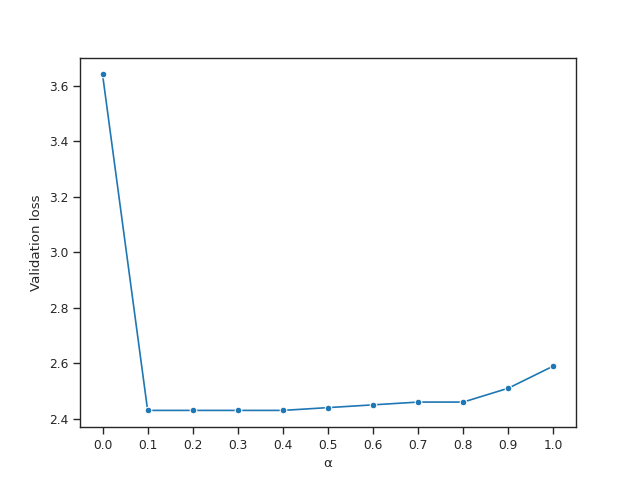
\includegraphics[scale=0.4]{pics/params_pruned_vs_val_loss-decoder.png}}
	\hfill
	\subfloat[Pruning en- and decoder]{\includegraphics[scale=0.4]{pics/params_pruned_vs_val_loss-both.png}}
	\caption[]{\label{fig:dev-performance}Pruning effects on the validation loss of the RGB auto-encoder on CARLA images.}
\end{figure}
\begin{figure*}[hbt]
	\centering
	\subfloat[Original image]{\includegraphics[scale=0.175]{pics/rgb_0_original.png}}
	\qquad
	\subfloat[Reconstructed image before pruning\label{fig:original_model_rgb_0_output}]{\includegraphics[scale=0.175]{pics/original_model_rgb_0_output.png}}
	\qquad
	\subfloat[Original image]{\includegraphics[scale=0.175]{pics/rgb_1_original.png}}
	\qquad
	\subfloat[Reconstructed image before pruning\label{fig:original_model_rgb_1_output}]{\includegraphics[scale=0.175]{pics/original_model_rgb_1_output.png}}
	\qquad
	\subfloat[Reconstructed image after pruning and before multiplication of weights (sim.)]{\includegraphics[scale=0.175]{pics/after_prun_before_mult_rgb_0_both.png}}
	\qquad
	\subfloat[Reconstructed image after pruning and after multiplication of weights (sim.)]{\includegraphics[scale=0.175]{pics/after_prun_after_mult_rgb_0_both.png}}
	\qquad
	\subfloat[Reconstructed image after pruning and before multiplication of weights (sim.)]{\includegraphics[scale=0.175]{pics/after_prun_before_mult_rgb_1_both.png}}
	\qquad
	\subfloat[Reconstructed image after pruning and after multiplication of weights (sim.)]{\includegraphics[scale=0.175]{pics/after_prun_after_mult_rgb_1_both.png}}
	\qquad
	\subfloat[Reconstructed image after pruning and before multiplication of weights (seq.)]{\includegraphics[scale=0.175]{pics/after_prun_before_mult_rgb_0.png}}
	\qquad
	\subfloat[Reconstructed image after pruning and after multiplication of weights (seq.)]{\includegraphics[scale=0.175]{pics/after_prun_after_mult_rgb_0.png}}
	\qquad
	\subfloat[Reconstructed image after pruning and before multiplication of weights (seq.)]{\includegraphics[scale=0.175]{pics/after_prun_before_mult_rgb_1.png}}
	\qquad
	\subfloat[Reconstructed image after pruning and after multiplication of weights (seq.)]{\includegraphics[scale=0.175]{pics/after_prun_after_mult_rgb_1.png}}
	\caption[]{Final results after pruning both, encoder and decoder of the RGB auto-encoder.
		First row shows original image and unpruned auto-encoder results.
		Second row shows results of pruning en- and decoder simultaneously (sim.).
		Third row shows results of pruning en- and decoder sequentially (seq.).
	}
	\label{fig:example_reconstructions}
\end{figure*}

\section{Conclusion}\label{sec:conclusion}
\subsection{Summary}
The goal of this paper was to prune different neural networks using a novel filter pruning framework for structured pruning with predefined target network architectures and without the need for fine-tuning.
It could be shown, that directly training the small target model from random initialization can achieve similar performance, as the model obtained from the standard pruning three-stage pipeline.
The best results have been achieved by allowing weight updates for the pre-trained model branch and increasing the learning rate as soon as local minima occur\footnote{Which is likely to happen once $\alpha$ is set equal to zero.}.
In all successful experiments an step-schedule with a step-size of 0.1 was used to schedule $\alpha$.
Other schedulers did not produce better results, indicating that the learning rate contributes much more to the success of this framework than $\alpha$.
Nonetheless, the question of the ideal schedule remains open.

\subsection{Outlook}
In order to answer open questions, the next logical step would be to execute both experiments with a larger step size.
Overall, it would be desirable if one could use the proposed approach to set $\alpha$ directly or very quickly to 0.1 or a similarly low value, to then continue with an exponential schedule, for example.
I am optimistic that something similar would be possible, since the intermediate models' performance did not change much during pruning in both experiments.\\
It would also make sense to further examine effects of so far unsuccessful attempts such as weight decay with a different decay-rate, though they were not further pursued, but could also help to achieve better results.\\
In parallel, the proposed pruning framework could be applied to other, more complex models, such as an auto-encoder with skip connections.
Another, more sophisticated network would be a DCGAN, whose architecture is similar to that of an auto-encoder.
Here, too, it would be interesting whether pruning the generator and discriminator separately or simultaneously makes a significant differance.

\clearpage
\onecolumn
{\small
%\bibliographystyle{ieee}
\bibliographystyle{plain}
\bibliography{bib}
}

\clearpage
\appendix
\section{Appendix}
\begin{table}[hpbt]
	\centering
	\begin{tabular}{ | l | l | l | }
		\hline
		\multicolumn{3}{|c|}{\textbf{RGB Auto-encoder}} \\
		\hline \hline
		Name & Type & Weight Shape \\ \hline \hline
		Conv0 & Conv2d & $64\times3\times3\times3$ \\ \hline
		Conv1 & Conv2d & $64\times64\times3\times3$ \\ \hline
		max\_pooling & MaxPool2d & - \\ \hline
		Conv2 & Conv2d & $128\times64\times3\times3$ \\ \hline
		Conv3 & Conv2d & $128\times128\times3\times3$ \\ \hline
		max\_pooling & MaxPool2d & - \\ \hline
		Conv4 & Conv2d & $128\times128\times3\times3$ \\ \hline
		Conv5 & Conv2d & $128\times128\times3\times3$ \\ \hline
		Conv6 & Conv2d & $128\times128\times3\times3$ \\ \hline
		max\_pooling & MaxPool2d & - \\ \hline
		\multicolumn{3}{|c|}{\textbf{bottleneck}} \\ \hline
		ConvTrans0 & ConvTranspose2d & $128\times128\times2\times2$ \\ \hline
		Conv7 & Conv2d & $128\times128\times3\times3$ \\ \hline
		Conv8 & Conv2d & $128\times128\times3\times3$ \\ \hline
		Conv9 & Conv2d & $128\times128\times3\times3$ \\ \hline
		ConvTrans1 & ConvTranspose2d & $128\times128\times2\times2$ \\ \hline
		Conv10 & Conv2d & $128\times128\times3\times3$  \\ \hline
		Conv11 & Conv2d & $128\times64\times3\times3$  \\ \hline
		ConvTrans2 & ConvTranspose2d & $64\times64\times2\times2$ \\ \hline
		Conv12 & Conv2d & $64\times64\times3\times3$ \\ \hline
		Conv13 & Conv2d & $64\times3\times3\times3$ \\ \hline
	\end{tabular}
	\caption{\label{appendix:architecture} Original RGB auto-encoder architecture.
		Each convolutional layer is followed by a BatchNorm and a ReLU activation.}
\end{table}
\begin{figure*}
	\centering
	\subfloat[Training accuracy]{\includegraphics[scale=0.5]{pics/train_acc.png}}
	\subfloat[Validation accuracy]{\includegraphics[scale=0.5]{pics/val_acc.png}}
	\caption[]{Accuracy development for selected $\alpha$-values using an exponential schedule with a decay-rate of 0.05.}
	\label{appendix:failed1}
\end{figure*}
\begin{figure*}
	\centering
	\subfloat[Training accuracy]{\includegraphics[scale=0.5]{pics/train_acc_DA.png}}
	\subfloat[Validation accuracy]{\includegraphics[scale=0.5]{pics/val_acc_DA.png}}
	\caption[]{Accuracy development for selected $\alpha$-values with data augmentation applied on half of the training data.}
	\label{appendix:failed2}
\end{figure*}
\begin{figure*}[hpbt]
	\centering
	\subfloat[Training accuracy]{\includegraphics[scale=0.75]{pics/weight_decay_train.png}}
	\subfloat[Validation accuracy]{\includegraphics[scale=0.75]{pics/weight_decay.png}}
	\caption[]{Accuracy development without weight decay (using a step decay) and with weight decay (using a weight decay-rate of 1e-4 and an exponential decay).}
	\label{appendix:failed4}
\end{figure*}


\end{document}
